\documentclass[xcolor=dvipsnames,18]{beamer}
%\usetheme{Madrid}
\usetheme {default}
\usepackage[ddmmyy]{datetime}
\usepackage{helvet}
\renewcommand{\familydefault}{\sfdefault}
\useinnertheme{rounded}
%fermilab color 
\definecolor{NALBlue}{RGB}{0, 76, 151} % UBC Blue (primary)
\definecolor{MARBlue}{RGB}{0, 181, 226} % UBC Blue (primary)
\definecolor{75Grey}{RGB}{99, 102, 106} % UBC Grey (secondary)

\definecolor{UBCgrey2}{RGB}{153, 214, 234} % UBC Grey (secondary) RGB: 153, 214, 234

\setbeamercolor{palette primary}{bg=NALBlue,fg=white} %
\setbeamercolor{structure}{fg=NALBlue} % itemize, enumerate, etc
%\setbeamercolor{normal text}{bg=NALBlue,fg=white}
\setbeamercolor{normal text}{fg=75Grey}
\setbeamercolor{author}{fg=NALBlue}
\setbeamercolor{date}{fg=NALBlue}
\setbeamercolor{footline}{fg=NALBlue}
\setbeamercolor{item}{fg=75Grey}





\setbeamertemplate{frametitle}
{
    \begin{beamercolorbox}[ht=1.2cm,rightskip=.3cm]{frametitle}
        \vbox{}\vskip-2ex%
        \strut\insertframetitle\strut
        \vskip-0.8ex%
        \color{UBCgrey2}\rule{1.05\linewidth}{1.5pt}
    \end{beamercolorbox}%

}


\setbeamertemplate{title page}[default][left]


\setbeamertemplate{title page}
{\vbox{}
    \begin{beamercolorbox}[sep=8pt,left]{title}
    
\includegraphics[width=5cm]{FNAL-Logo-NAL-Blue.png}
    {\color{UBCgrey2}\rule{1\linewidth}{1.5pt}}
      \tiny Managed by Fermi Research Alliance, LLC for the U.S Department of Energy Office of Science
      
      
      {\color{UBCgrey2}\rule{1\linewidth}{1.5pt}}
    \end{beamercolorbox}
    \begin{beamercolorbox}[sep=8pt,left]{author}
    \usebeamerfont{title}\inserttitle
    \end{beamercolorbox}
    \begin{beamercolorbox}[sep=8pt,left]{author}
     \usebeamerfont{author}\insertauthor 
     \vspace{0.25cm}
     \usebeamerfont{author}\insertinstitute \\
     \vspace{0.25cm}
     \insertdate
    \end{beamercolorbox}
    %\vskip-1em\par % change here
}
    


    
\setbeamercolor{palette secondary}{bg=MARBlue,fg=white}
\setbeamercolor{palette tertiary}{bg=75Grey,fg=white}
%\setbeamercolor{palette quaternary}{bg=UBCblue,fg=white}
\setbeamercolor{author in head/foot}{bg=NALBlue,fg=white}     
\setbeamercolor{institute in head/foot}{bg=NALBlue,fg=white}  
%\setbeamercolor*{title}{bg=NALBlue,fg=white}          

\setbeamercolor{subsection in head/foot}{bg=NALBlue,fg=white}

\setbeamertemplate{footline}{
   %\dsglogo
   \begin{beamercolorbox}[ht=5pt,leftskip=1cm,rightskip=.3cm]{}
    %\hrule
    {\color{UBCgrey2}\rule{0.7\linewidth}{4pt}}
    \hfill
    \raisebox{-0.8mm}{
\includegraphics[width=2cm]{FNAL-Logo-NAL-Blue.png}}
    \newline
    %\vspace{0.25cm}
    \scriptsize \insertframenumber \hspace{0.5cm} \insertdate \hspace{0.5cm} \insertshortauthor \hspace{0.2cm} \vrule width 0.75pt \hspace{0.2cm}
  \insertshorttitle 
    \newline
    %\insertshortauthor \ - \insertshortinstitute \hfill \insertframenumber
   \end{beamercolorbox}
   \vspace*{0.1cm}
} 

\beamertemplatenavigationsymbolsempty


\title[Transverse Instabilities at FNL ]{Transverse Instabilities at the FermiLab Recycler Ring}

\author[O.Mohsen]
{Osama Mohsen}
\institute[s]{test}
\date{\today}

\begin{document}
\begin{frame}
\titlepage
\end{frame}
\begin{frame}{Review}
    \tableofcontents
\end{frame}
\section{Transverse Instabilities}
\subsection{Wake field, Impedance and space charge}
\begin{frame}{Wake fields}
\begin{columns}[T] % align columns
\begin{column}{.48\textwidth}
%\color{red}\rule{\linewidth}{4pt}
\begin{itemize}
    \item Wake fields are electromagnetic fields self-generated by the beam interaction with its surrounding (e.g. metallic structures, vacuum chambers, plasma) 
    \item The impedance is related to the FT of the wake fields. 
\end{itemize}
\end{column}%
\hfill%
\begin{column}{.48\textwidth}
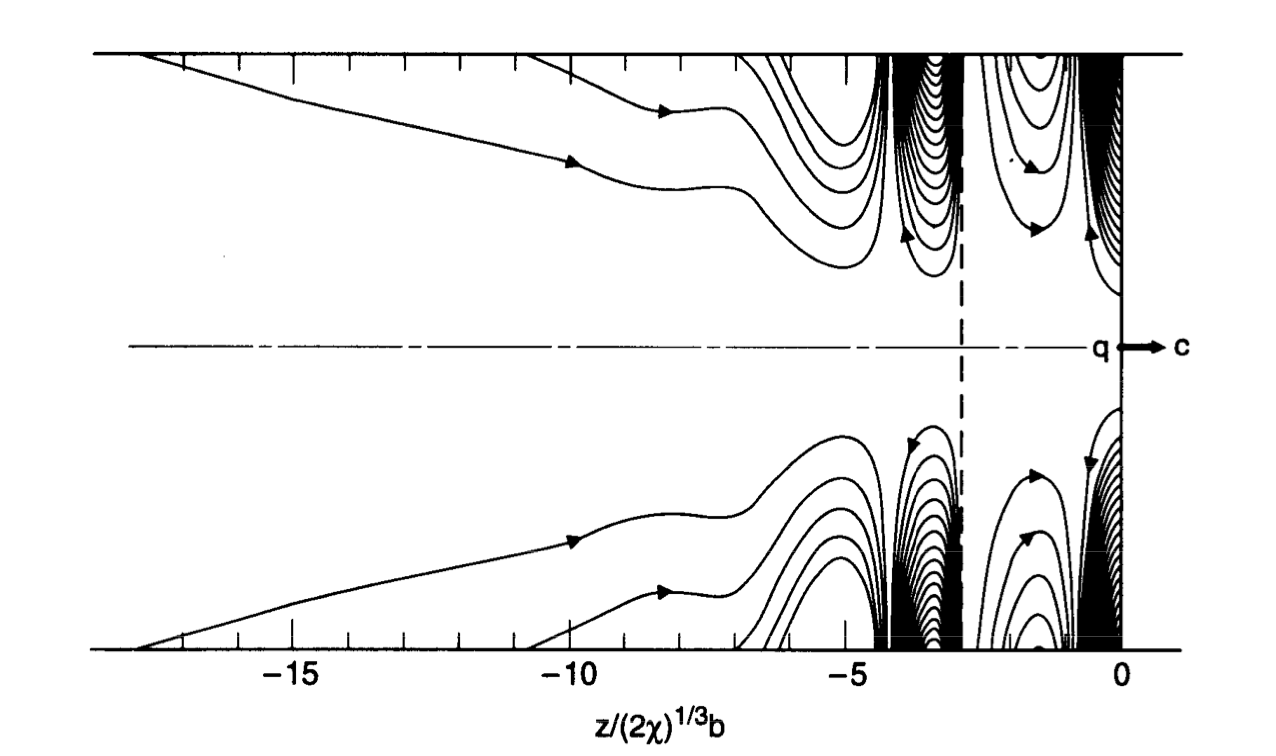
\includegraphics[width=1\linewidth]{pic/Wake.png}
\end{column}%
\end{columns}
\end{frame}
\begin{frame}{Space Charge}
\begin{columns}[T] % align columns
\begin{column}{.48\textwidth}
%\color{red}\rule{\linewidth}{4pt}
\begin{itemize}
    \item Space Charge (SC) is the force experienced by the beam due to the individual particle field. Space Charge is an N-body problem but can be treated as a collective effect and can be treated as an Impedance. 
\end{itemize}
\end{column}%
\hfill%
\begin{column}{.48\textwidth}
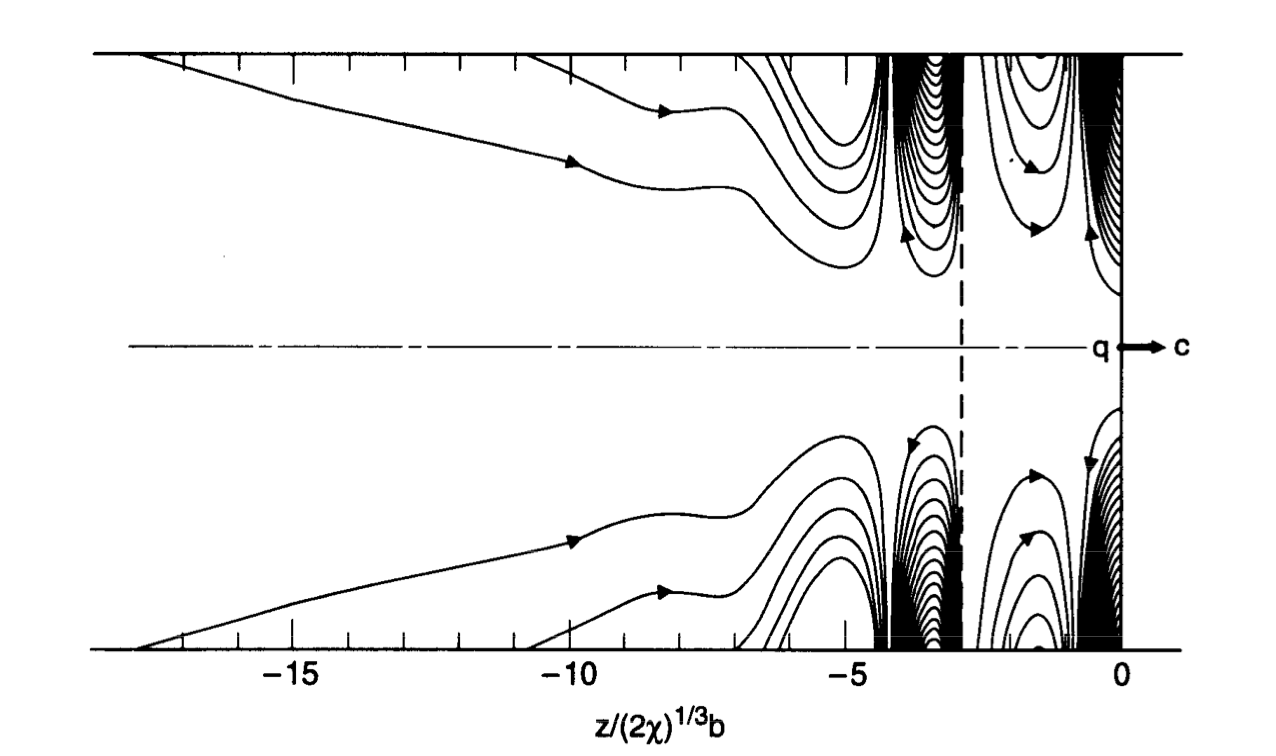
\includegraphics[width=1\linewidth]{pic/Wake.png}
\end{column}%
\end{columns}
\end{frame}
\subsection{Instabilities}
\begin{frame}{Instabilities}
Wake fields generated by the beam due to its interaction with surroundings will act back on the beam as a perturbation. If the conditions are correct, this perturbation can grow in time and causes the beam to become unstable. This translates, in operation, to beam losses and intensity limits.  Studying these instabilities help predict and mitigate them. 
\end{frame}
\subsection{Transverse Mode Coupling Instability (TMCI)}
\begin{frame}{Frame Title}
\begin{columns}
\begin{column}{0.45\textwidth}
\centering
\begin{itemize}
    \item Item 1
    \item Item 2
\end{itemize}
\end{column}
\begin{column}{0.45\textwidth}
\centering

\includegraphics[width=1\linewidth]{FNAL-Logo-NAL-Blue.png}\\
\end{column}
\end{columns}
\end{frame}
\section{FermiLab Accelerator Complex}
\begin{frame}{Frame Title}
\end{frame}
\section{The waker system}
\begin{frame}{Frame Title}
\end{frame}

\section{Recent progress}
\begin{frame}{Frame Title}
\end{frame}

\section{moving forward}
\begin{frame}{Frame Title}
\end{frame}

\end{document}